Si è deciso di utilizzare il servizio di gestione dei \gls{task} e creazione di \gls{milestone} offerto da \gls{GitHub}. Questo permette di accentrare le informazioni in un solo ambiente.\\

\subsection{Creazione e gestione dei ticket}

I \gls{ticket} vengono creati e gestiti quasi tutti dal responsabile di progetto.
Qualora il \textit{Verificatore} trovasse imprecisioni o errori durante la verifica, avrà la possibilità di creare dei \gls{ticket} per segnalare suddetti errori.
Ogni \gls{ticket} può essere assegnato ad uno o più membri del gruppo a seconda della complessità del lavoro e della disponibilità dei membri del gruppo.
Per creare un nuovo \gls{ticket} bisogna:

\begin{itemize}
	\item Posizionarsi alla voce Issue;
	\item Premere "New issue";
	\item Compilare i campi richiesti:
		\begin{itemize}
			\item \textbf{Titolo e commenti:} titolo descrittivo con una descrizione del nuovo \gls{ticket};
			\item \textbf{Labels:} dovranno avere due caratteristiche fondamentali e cioè la tipologia di \gls{ticket} assegnato(modifica, verifica, richiesta approvazione) e la priorità assegnata(alta, media, bassa);
			\item \textbf{\gls{Milestone}:} la \gls{milestone} a cui è associato il \gls{ticket};
			\item \textbf{Assignee:} a chi viene assegnato il \gls{ticket}.
		\end{itemize}
\end{itemize}
\begin{figure}[h]
\centering
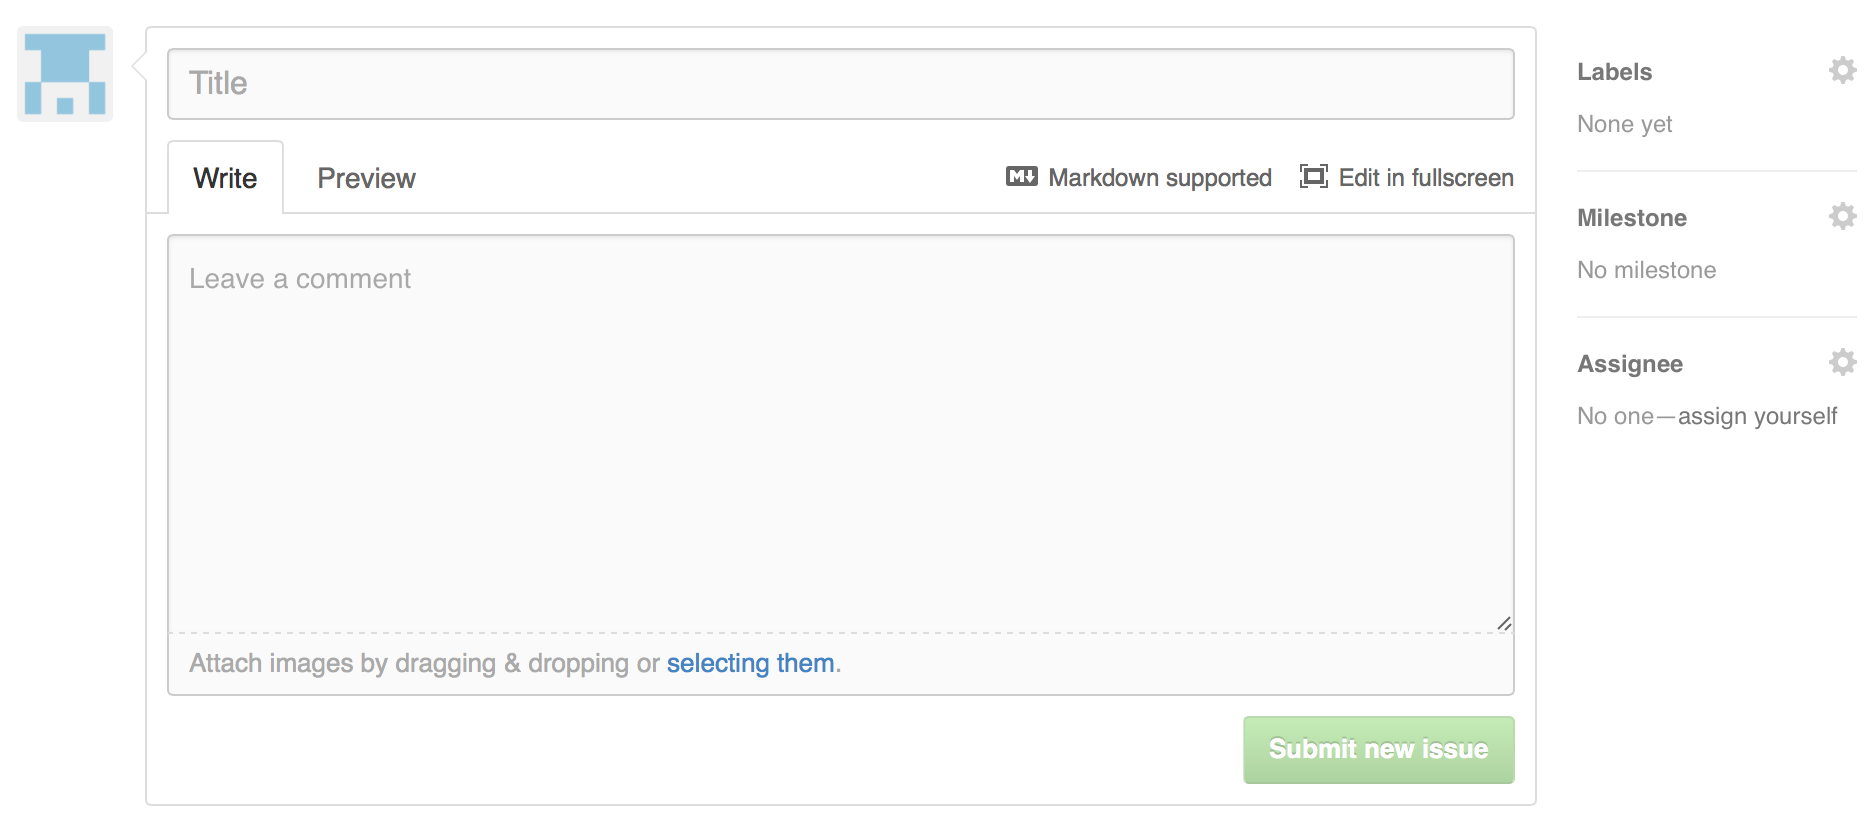
\includegraphics[width=0.7\linewidth]{img/ticket}
\caption[Creazione ticket]{Creazione \gls{ticket}}
\label{fig:ticket}
\end{figure}


\subsection{Creazione delle milestone}

Il responsabile di progetto ha il compito della creazione di una \gls{milestone} in occasione di ogni revisione al quale il gruppo \GRUPPO\ ha intenzione di partecipare, più altre \gls{milestone} qualora il responsabile di progetto lo ritenga necessario.

Per creare una nuova \gls{milestone} bisogna:

\begin{itemize}
	\item Posizionarsi alla voce \gls{Milestone};
	\item Premere "New \gls{milestone}";
	\item Compilare i campi richiesti:
		\begin{itemize}
			\item \textbf{Titolo;}
			\item \textbf{Descrizione;}
			\item \textbf{Data.}
		\end{itemize}
\end{itemize}
\begin{figure}[h]
\centering
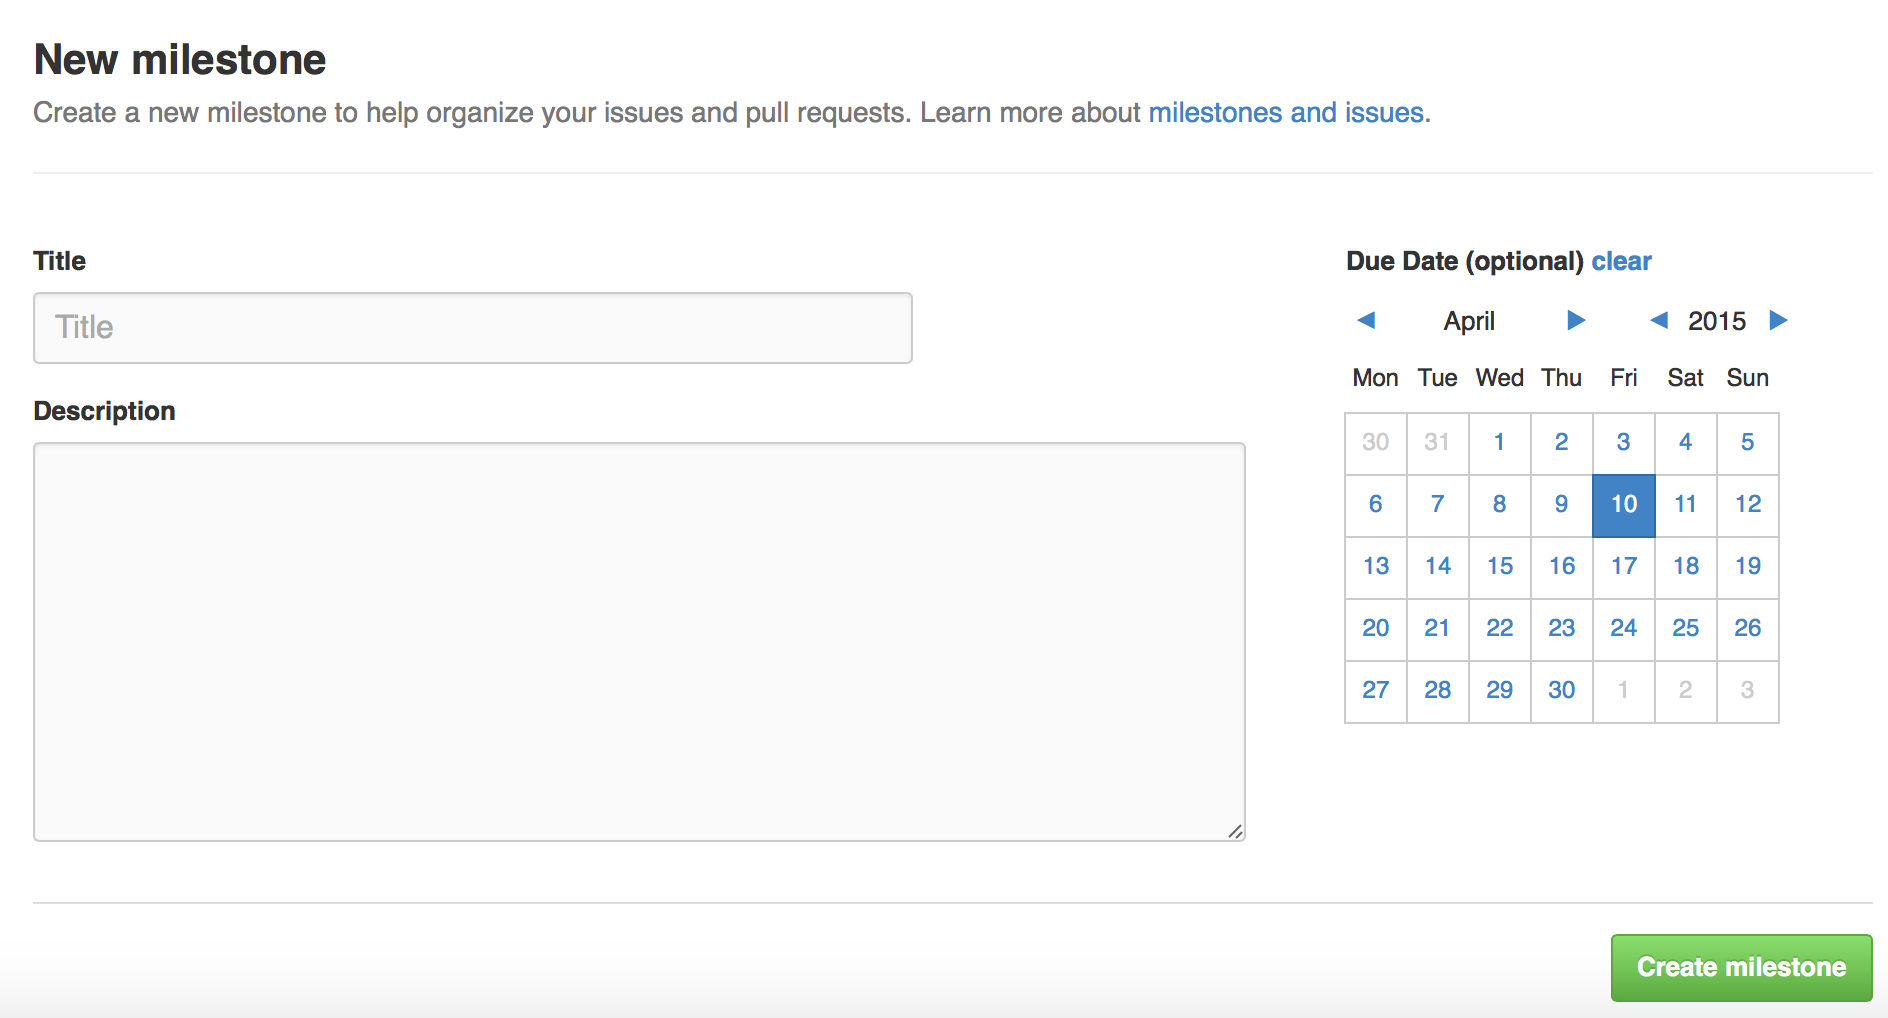
\includegraphics[width=0.7\linewidth]{img/milestone}
\caption[Creazione milestone]{Creazione milestone}
\label{fig:milestone}
\end{figure}


\subsection{Esecuzione dei compiti}

Ogni membro del gruppo è tenuto a visionare regolarmente la presenza di \gls{ticket} a lui assegnati e segnalarne la presa in consegna.
Una volta che un membro porta a termine un \gls{ticket} deve modificarne lo stato per segnalare il termine del lavoro.
Se un \gls{ticket} non ha avuto i risultati attesi il \textit{Responsabile di Progetto} può riaprirlo ed eventualmente assegnare altri membri al lavoro.

\subsection{Chiusura della milestone}

Una volta raggiunta la scadenza, il \textit{Responsabile di Progetto}, deve chiudere la \gls{milestone} ed eventualmente aprirne un'altra per poi ricominciare tutto il protocollo da capo.

